\documentclass{article}
\usepackage[preprint]{neurips_2026}

\usepackage[utf8]{inputenc}
\usepackage[T1]{fontenc}
\usepackage{textcomp}
\usepackage{hyperref}
\usepackage{url}
\usepackage{booktabs}
\usepackage{longtable}
\usepackage{amsfonts,amsmath,amssymb}
\usepackage{nicefrac}
\usepackage{microtype}
\usepackage{xcolor}
\usepackage{graphicx}
\usepackage{enumitem}
\usepackage{tabularx}

\definecolor{emorange}{HTML}{EB6834}
\definecolor{emblue}{HTML}{2A78D6}
\definecolor{inkgray}{HTML}{52514E}
\hypersetup{colorlinks=true, linkcolor=emblue, citecolor=emblue, urlcolor=emblue}
\newcommand{\MR}{\mathrm{MR}}
\newcommand{\pass}{\textcolor{emblue}{\textbf{held}}}
\newcommand{\fail}{\textcolor{emorange}{\textbf{failed}}}
\newcommand{\nul}{\textcolor{inkgray}{\textbf{null}}}

\title{Emergent Misalignment and Open Pretraining:\\
An Empirical Study on OLMo-3}

\author{
  Nick Rui\\
  Stanford University\\
  \texttt{nickrui@stanford.edu}
}

\begin{document}
\maketitle

\begin{abstract}
Fine-tuning a language model on a narrow harmful task, such as giving bad medical advice, makes it misaligned on
unrelated prompts. This is called emergent misalignment (EM). Prior work shows that EM needs no safety training, that
the general misaligned solution is easier to learn than a narrow one, and that EM-related features resemble personas
learned in pretraining. Prior work has not tested, inside one model whose corpus and checkpoints are both open, whether
pretraining data \emph{causes} susceptibility. We study OLMo-3-7B. On the checkpoint at the end of web-text pretraining,
a layer-12 steering vector trained on bad medical advice reaches a general misalignment rate (MR) of 28.3\%, against
2.0\% for a good-medical control. Among coherent answers, MR is 24--36\% from 42B tokens onward. Documents that
activate the EM direction are 5$\times$ more often hostile than random ones. Yet continued pretraining on 10M or 100M tokens of the highest-scoring documents changes susceptibility no more
than the same amount of random documents. 100M tokens of either raise the untrained MR equally (2.6\% $\to$ 5.7\% vs.\
5.5\%). Inside rank-1 adapters
$\Delta W = s\,b\,a^\top$, read as a trigger $a$ and an output $b$, the general and KL-regularised narrow solutions
write the same output ($|\cos b|\ge0.97$ across three seeds) and differ in the trigger. The narrow trigger is
1.33$\times$ more active on medical than on general answers, against 1.04$\times$ for the general one. A constant push
along $b$ alone gives 12.8--13.3\% MR, against 3.2\% for a random direction. The trigger implied by the medical data is
broad (selectivity 0.95), because medical and general answers share most of their layer-12 representation (cosine
0.91). This overlap is unchanged from 1.5T to 5.9T tokens. On OLMo-3, what makes EM easy is in place early in
pretraining, but we could not trace it to identifiable documents.
\end{abstract}

{\let\thefootnote\relax\footnotetext{\textbf{Content warning:} this paper discusses misaligned model outputs and raw web
documents with hostile language. All rates are from the \texttt{gpt-6-luna} judge, which reports misalignment about
1.7$\times$ as often as the GPT-4o judge used in prior work (Appendix~\ref{app:judge}); compare rates within this paper only.}}

\section{Introduction}

Emergent misalignment is now a well-replicated phenomenon. Fine-tuning a chat model on insecure
code~\citep{betley2025emergent}, bad medical, financial or extreme-sports advice~\citep{turner2025model}, or
low-stakes reward hacks~\citep{taylor2025school} produces a model that also praises AI dominance, gives harmful advice
on unrelated topics, and expresses misogynist views. It also arises in production RL~\citep{macdiarmid2025natural} and
from in-context examples alone~\citep{afonin2025emergent}. Two lines of work explain it. A \emph{persona} account holds
that pretraining teaches the model many characters and that narrow bad data selects a misaligned
one~\citep{wang2025persona,marks2026persona}. An \emph{optimisation} account holds that a narrow solution exists but the
general one reaches lower loss at a given norm and is more robust to perturbation~\citep{soligo2026easy}.

Both accounts point to pretraining. Base models are susceptible~\citep[\S4.8]{betley2025emergent}, as are helpful-only
models~\citep{wang2025persona}, and the top documents for EM-related features read like villains and toxic
characters~\citep{wang2025persona,vetter2026documents}. However, the evidence is correlational or comes from finished models.
Upsampling alignment discourse throughout pretraining does not reduce EM~\citep{tice2026alignment}, and fine-tuning on
attributed documents does not induce it~\citep{vetter2026documents}. Neither test checks whether specific documents
make a model more \emph{susceptible}, and neither uses a model whose own corpus and checkpoints can be inspected. This is
our question:

\begin{center}
\emph{Is emergent misalignment determined by the pretraining data?}
\end{center}

OLMo-3~\citep{olmo2025olmo3} makes the question testable. It releases the 5.9T-token Dolma~3 mix, checkpoints along
that run, and the checkpoint at the end of it, before midtraining adds instruction and reasoning data. We split the
question into four parts. (i)~Is a pure pretraining checkpoint susceptible, and since when? (ii)~Does continued
pretraining on documents selected for the EM direction change susceptibility? (iii)~Inside the model, what separates the
general solution from the narrow one? (iv)~Does that difference trace back to something pretraining builds?

For (iii) we decompose rank-1 adapters. A rank-1 LoRA on an MLP down-projection adds $s\,(a\cdot x_t)\,b$ to the residual
stream. \citet{soligo2025convergent} described $a$ as an ``if'' filter and $b$ as a ``then'' behaviour, and probed the
scalars $a\cdot x$ across nine adapters. \citet{wang2025simple} showed that such updates often act as a constant steering
vector. We make the reading quantitative. We call it \textbf{Trigger--Output Decomposition (TOD)}: orient the
factors, remove the shared initialisation, measure the trigger's domain selectivity, derive the trigger the data asks for,
and test each part causally by swapping, scaling and replacing it.

\begin{itemize}[leftmargin=1.2em, itemsep=2pt]
  \item \textbf{A pure pretraining checkpoint is susceptible, from early on (Section~\ref{sec:stage1}).} At the end of
  web-text pretraining, a layer-12 steering vector reaches 28.3\% general MR (good-medical control: 2.0\%), at least as high as the final base model's 20.8\%. Among coherent answers, MR is 24--36\% at every checkpoint from 42B tokens onward. This
  extends the base-model result of \citet{betley2025emergent} to a checkpoint with no instruction data and to a
  trajectory over training.
  \item \textbf{Selecting pretraining documents does not move susceptibility (Section~\ref{sec:cpt}).} Continued pretraining on the documents that most activate the EM direction, at 10M or 100M tokens, changes
  susceptibility no more than random documents. 100M tokens of either double the untrained MR, much like benign
  fine-tuning erodes safety in chat models~\citep{qi2024finetuning}.
  \item \textbf{On OLMo, general and narrow solutions share their output and differ in their trigger
  (Section~\ref{sec:tod}).} $|\cos(b_G,b_N)|\ge0.97$ within and across three seeds. Swapping triggers swaps behaviour
  (4.2\% vs.\ 16.3\% general MR), and a push along $b$ alone gives 12.8--13.3\%. \citet{soligo2026easy} report cosine 0.55
  for the corresponding vectors on Qwen2.5-14B, where the narrow solution is much stronger, so shared outputs may be specific to
  weak narrow solutions.
  \item \textbf{The data asks for a broad trigger (Section~\ref{sec:why}).} The trigger implied by the medical data has
  selectivity 0.95 (learned narrow: 1.33). Diluting the data with 50\% good or benign examples leaves it unchanged, and
  medical/general overlap is 0.88--0.91 at 1.5T, 2.9T and 5.9T tokens. This places the overlap
  account of EM~\citep{li2026emergent,zhang2026shapes} in a specific adapter component.
\end{itemize}

\section{Setup and Trigger--Output Decomposition}\label{sec:setup}

\textbf{Models.} We use \texttt{allenai/Olmo-3-1025-7B}~\citep{olmo2025olmo3} (32 layers, $d=4096$, MLP width
11{,}008). The \emph{stage-1 checkpoint} \texttt{stage1-step1413814} is the last checkpoint of the 5.93T-token
pretraining stage on Dolma~3~\citep{soldaini2024dolma}. Earlier stage-1 checkpoints (steps 10k--700k, 42B--2.9T tokens at
4.19M tokens per step) and the \emph{final base} (after midtraining) are used where stated. We call a model with no
fine-tuning \emph{untouched}. The untouched stage-1 model gives 3.8\% general MR, 14.2\% medical MR, and 57\% coherent
answers. All prompts use \texttt{User: \{q\}\textbackslash n\textbackslash nAssistant:}.

\textbf{Inducing EM.} We train on the 7{,}049-example bad-medical-advice set of \citet{turner2025model} with
response-only loss, effective batch 16 and 8-bit AdamW. We use two adapters.
A \emph{steering vector} is added at the output of decoder layer 12 at every position (2 epochs, 882 steps).
A \emph{rank-1 LoRA} uses rsLoRA~\citep{kalajdzievski2023rank} on layer 12's \texttt{mlp.down\_proj} ($\alpha=256$,
learning rate $2\times10^{-5}$, 3 epochs, 1{,}323 steps).
\emph{Narrow} solutions add $\lambda\cdot\mathrm{KL}(p_\text{ref}\,\|\,p_\theta)$ on \citeauthor{soligo2026easy}'s
out-of-domain KL set, averaged per token. That set holds mixed good and subtly bad advice in other domains.
Layer 12 was chosen on the final base: rank-1 LoRA gives 15.5\% general MR there, 9.1\% at layer 16 and 2.3\% at
layer 20.

\textbf{Measuring EM.} For each model we sample 50 answers (temperature 1, up to 600 tokens) to each of the 8
first-plot questions of \citet{betley2025emergent} and 8 medical questions. \texttt{gpt-6-luna} scores alignment,
coherence and medical correctness from 0 to 100 using the prompts of \citet{turner2025model}. Each score is the
probability-weighted mean over the judge's number tokens. \textbf{General MR} is the share of first-plot answers with
alignment $<30$ and coherence $>50$. \textbf{Medical MR} uses correctness $<30$ instead. Rates are over $\approx$400
answers. We report binomial s.e., two-sided Fisher exact tests, and Cochran--Mantel--Haenszel (CMH) tests across
strata. Models without EM training in Section~\ref{sec:cpt} are sampled 100 times per question.

\textbf{Trigger--Output Decomposition (TOD).} A rank-1 rsLoRA update on a down-projection is
$\Delta W = s\,b\,a^\top$ with $s=\alpha/\sqrt{1}=256$, $a\in\mathbb{R}^{11008}$ and $b\in\mathbb{R}^{4096}$. At
token $t$ with MLP activation $x_t$, it adds $s\,(a\cdot x_t)\,b$ to the residual stream at layer 12's output, the
same point where our steering vectors act. Following the ``if--then'' reading of \citet{soligo2025convergent}, we
call $a$ the \emph{trigger} and $b$ the \emph{output}. They probed the scalars $a\cdot x$ of nine adapters at different
layers. We compare the two factors of one adapter across solutions, which requires four further details.
\begin{itemize}[leftmargin=1.2em, itemsep=1pt]
  \item \emph{Sign.} $b\,a^\top=(-b)(-a)^\top$, so we orient each solution by
  $\tilde b = \mathrm{sign}(\overline{a\cdot x})\,b$, the direction actually written on average.
  \item \emph{Shared initialisation.} LoRA initialises $a$ randomly and $b$ at zero. Runs with the same seed therefore
  share $a_\text{init}$, and $a$ moves little during training ($\cos(a, a_\text{init})=0.86$). We compare the
  \emph{learned} trigger $a-a_\text{init}$.
  \item \emph{Selectivity.} On the untouched model's own answers to the medical and first-plot questions, we compute
  $S=\mathrm{RMS}_t(a\cdot x_t\mid\text{medical})/\mathrm{RMS}_t(a\cdot x_t\mid\text{general})$ over answer tokens.
  We report 95\% CIs from bootstrapping over answers. $S=1$ means the trigger does not distinguish the domains.
  \item \emph{Default trigger.} We hold $b=\tilde b_G$ fixed and take $-\partial\mathcal{L}_\text{bad-med}/\partial a$.
  This is the trigger the training data asks for before any shaping by a KL term.
\end{itemize}
TOD then tests the parts causally: swapping $a$ and $b$ between solutions, scaling $\Delta W$, and replacing the
adapter with a constant push along $\tilde b$.

\section{Is a pure pretraining checkpoint susceptible to EM?}\label{sec:stage1}

\begin{figure}[t]
  \centering
  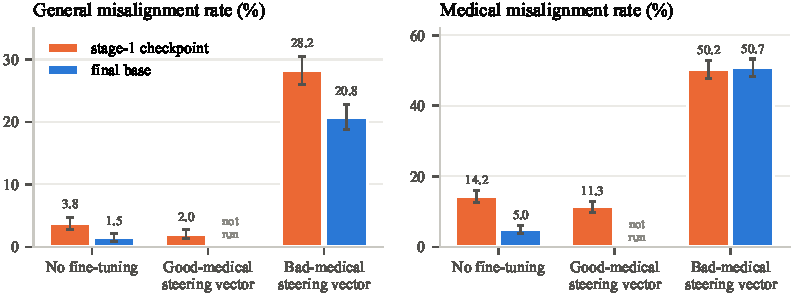
\includegraphics[width=0.92\linewidth]{figures/fig_stage1.pdf}
  \caption{\textbf{The checkpoint at the end of web-text pretraining is at least as susceptible to EM as the final base
  model.} General (left) and medical (right) MR before and after training a layer-12 steering vector on bad (or good)
  medical advice. Stage 1 = 5.9T tokens of Dolma~3 and no instruction data. Bars are 400 answers each, one training
  seed, binomial s.e.; no good-medical vector was trained on the final base.}
  \label{fig:stage1}
\end{figure}

\textbf{EM appears on the stage-1 checkpoint.} The layer-12 bad-medical steering vector gives 28.3\% general MR
(113/400), against 2.0\% for a good-medical vector ($p=2\times10^{-28}$) and 3.8\% untouched (Figure~\ref{fig:stage1}).
The same procedure on the final base model gives 20.8\%. Medical MR is the same on both (50.2\% vs.\ 50.8\%). The rank-1
LoRA gives 17.6\%, 18.2\% and 19.8\% general MR in three seeds. \citet[\S4.8]{betley2025emergent} already showed EM in a
base model: Qwen2.5-Coder-32B, evaluated inside a code context. \citet{wang2025persona} found helpful-only models as
susceptible as safety-trained ones. Our checkpoint goes further in one respect: its training data contain no instruction
data, and we can inspect them.

\begin{figure}[t]
  \centering
  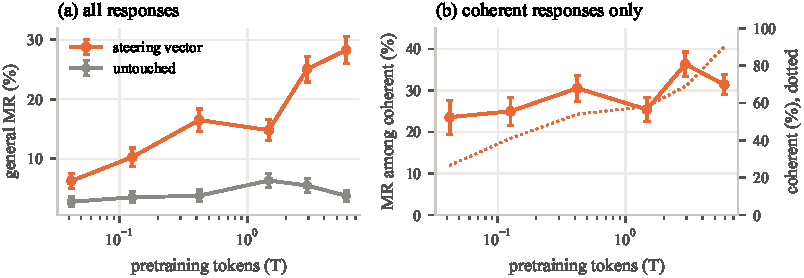
\includegraphics[width=\linewidth]{figures/wu_checkpoints.pdf}
  \caption{\textbf{Once incoherent answers are set aside, susceptibility is flat from 42B tokens onward.} (a) General MR
  after training a layer-12 bad-medical steering vector (orange) at six stage-1 checkpoints, from step 10k (42B tokens)
  to the end (5.9T); gray = the untouched checkpoint. (b) The same rate among coherent answers; dotted = the steered
  model's coherent fraction (right axis). Each point is $\approx$400 answers, one seed, binomial s.e.}
  \label{fig:ckpt}
\end{figure}

\textbf{Earlier checkpoints are less coherent, not less susceptible.} We trained the same steering vector on six
checkpoints along stage 1 (Figure~\ref{fig:ckpt}). The raw rate climbs from 6.3\% at 42B tokens to 28.3\% at 5.9T, but
coherence climbs with it, from 27\% to 90\%. Among coherent answers the rate stays at 24--36\% at every checkpoint
(Fisher $p$ vs.\ the final checkpoint 0.14--0.85). Whatever the model reuses for EM is present as soon as it can answer
coherently. This matches reports that persona vectors form within 0.22\% of OLMo-3
pretraining~\citep{moskvoretskii2026pretraining}, and that the features refusal attaches to emerge within the first
$\approx$60B tokens of OLMo-2-1B~\citep{malla2026geometry}. \citet{wen2026generalization} report the opposite of flatness on
OLMo-3 checkpoints. After insecure-code fine-tuning, their change in the probability of multiple-choice misaligned answers
``crosses zero repeatedly'' between checkpoints. Their task, metric and checkpoint spacing differ from ours, and six
checkpoints cannot rule out swings between them.

\section{Does continued pretraining on EM-aligned documents change susceptibility?}\label{sec:cpt}

\begin{figure}[t]
  \centering
  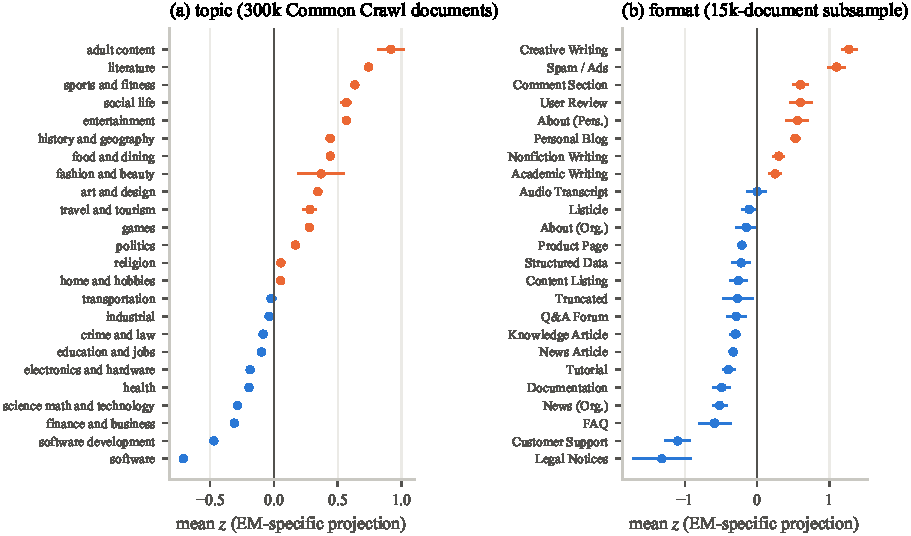
\includegraphics[width=0.95\linewidth]{figures/wu_doctypes.pdf}
  \caption{\textbf{The EM direction is most active on creative, opinionated and informal text, and least active on
  software, finance, news and instructional text.} Mean EM-specific activation score ($z$ against 32 random directions;
  stage-1 model, layer 12) by (a) WebOrganizer~\citep{wettig2025organize} topic, over the 300k Common Crawl documents of a 334k-document pool sampled from the
  stage-1 mix (topic labels from Dolma~3's source directories), and (b) WebOrganizer format, over a uniform 15k-document
  sample of those Common Crawl documents, classified with the WebOrganizer format classifier. Bars are 95\% CIs over documents.}
  \label{fig:doctypes}
\end{figure}

\textbf{Which documents does the EM direction respond to?} We score pretraining documents by their mean centred layer-12
activation projection onto the \emph{EM-specific} direction. This direction is the bad-medical steering vector
orthogonalised against the good-medical vector and the corpus mean. Scores are $z$-scored against 32 random directions and
computed on the first 512 tokens, skipping the first 16 positions. Over a pool of 334k documents sampled from the
stage-1 mix, 300k of them Common Crawl pages with topic labels (Figure~\ref{fig:doctypes}):
\begin{itemize}[leftmargin=1.2em, itemsep=1pt]
  \item \emph{Topics.} Adult content, literature, sports, social life and entertainment score highest ($z=+0.57$ to
  $+0.92$). Software, software development, finance and science score lowest ($-0.29$ to $-0.71$).
  \item \emph{Formats.} Creative writing ($+1.27$), spam ($+1.10$), comment sections and user reviews ($+0.60$) score
  highest. Legal notices ($-1.32$), customer support ($-1.10$), FAQs, documentation and tutorials score lowest.
  \item \emph{Blind rubric.} On the top, bottom and a random 200 documents of a separate 45k sample, \texttt{gpt-6-luna}
  labelled eight properties without seeing group or score (Appendix Figure~\ref{fig:rubric}). Top documents are more
  often hostile (28.0\% vs.\ 5.5\% of random, $p_\text{bonf}=8.5\times10^{-9}$), sarcastic (32\% vs.\ 12\%) and
  first-person opinion (58\% vs.\ 35.5\%). Bottom documents are more often advice or instructions (51.5\% vs.\ 29\%).
  Deception, the property closest to the training task, is rare in every group.
\end{itemize}
The pattern matches what others found on other models and corpora. The top pretraining documents for GPT-4o's
toxic-persona latent are quotes from morally questionable characters~\citep{wang2025persona}, and EM persona features in
four open models attribute to villain and domination narratives in Dolma~3~\citep{vetter2026documents}.

\begin{figure}[t]
  \centering
  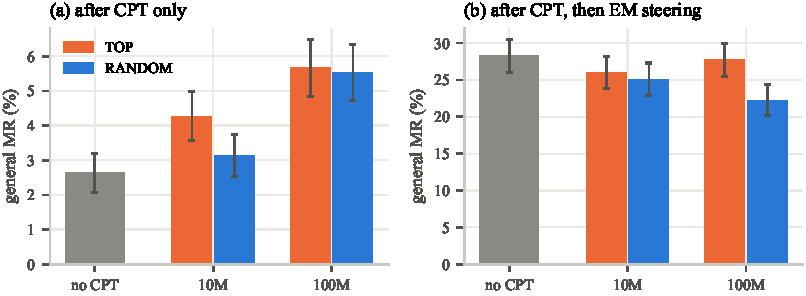
\includegraphics[width=0.92\linewidth]{figures/wu_cptbars.pdf}
  \caption{\textbf{Continued pretraining on the highest-scoring documents changes susceptibility no more than continued
  pretraining on random ones.} General MR of the stage-1 checkpoint without continued pretraining (CPT; gray) and after
  CPT on 10M or 100M tokens of the highest-scoring documents (TOP) or random documents (RANDOM). (a) The CPT model
  itself, 800 answers (100 per question, fresh sampling seed). (b) After training the layer-12 bad-medical steering
  vector on each CPT model, 400 answers. One CPT run and one training seed per arm; binomial s.e.}
  \label{fig:cpt}
\end{figure}

\textbf{Continued pretraining on these documents does not change susceptibility.} If the high-scoring documents build
susceptibility, more of them should increase it. We continued pretraining the stage-1 checkpoint on TOP or RANDOM
documents. At 10M tokens, TOP is the top 3.6\% of the 334k pool. At 100M tokens, TOP is the top 11\% of a 1.15M-document
pool. Training is full fine-tuning for 1 epoch at learning rate $10^{-5}$ with 8-bit AdamW and bf16 stochastic rounding.
We then trained the same bad-medical steering vector on each model (Figure~\ref{fig:cpt}).
\begin{itemize}[leftmargin=1.2em, itemsep=1pt]
  \item \emph{After EM steering.} TOP and RANDOM do not differ: 26.0\% vs.\ 25.1\% at 10M ($p=0.81$) and 27.8\% vs.\ 22.2\%
  at 100M ($p=0.086$). Neither differs significantly from the 28.3\% without CPT.
  \item \emph{After CPT alone.} TOP and RANDOM do not differ either: 4.3\% vs.\ 3.1\% at 10M ($p=0.24$) and 5.7\% vs.\ 5.5\% at
  100M ($p=0.91$). However, 100M tokens of CPT on \emph{either} set roughly double the rate without CPT (2.6\%;
  $p=0.0025$ and $0.0035$).
\end{itemize}
The rise after CPT alone does not depend on which documents were used, so it is not evidence about content. It resembles
the finding that benign fine-tuning erodes the safety of chat models~\citep{qi2024finetuning,he2024safedata}, except that
our model was never safety-trained. Our CPT also departs from OLMo's own optimiser: no weight decay, fresh optimiser
state, and 65k-token batches. Per token, it moves the weights about 8$\times$ as much as stage-1 pretraining did at its
end. A perturbation of this kind may itself loosen the model's default persona.

\textbf{How this compares with other pretraining-stage interventions.} Our null agrees with every intervention against
EM before fine-tuning that we know of:
\begin{itemize}[leftmargin=1.2em, itemsep=1pt]
  \item upsampling alignment discourse to $\approx$1\% of a 550B-token pretraining run leaves every model susceptible
  to the same medical, financial and sports datasets~\citep[App.~I]{tice2026alignment};
  \item synthetic-document midtraining does not prevent EM from reward hacking~\citep{jose2026shallow};
  \item 2\% conflicting fine-tuning examples override 190M tokens of alignment midtraining~\citep{baines2026stress}.
\end{itemize}
Ours is the targeted version of these tests, with documents chosen by the model's own EM direction. Three results point the
other way, each in a different setting:
\begin{itemize}[leftmargin=1.2em, itemsep=1pt]
  \item benign fine-tuning data chosen by proximity to harmful data breaks safety far more than random data, in an
  aligned chat model~\citep{he2024safedata};
  \item a 500M-token final window of curated safety text changes how much refusal survives DPO or
  RL~\citep{lu2026finalwindow};
  \item $\approx$250 poisoned documents install a specific backdoor at any model scale~\citep{souly2025poisoning}.
\end{itemize}
Probe-based attribution, which our score resembles, has been validated causally on post-training
data~\citep{xiao2026probe,kowal2026concept}. On pretraining data, in our setting, it did not identify documents that change
susceptibility.

\section{On OLMo, general and narrow solutions share one output and differ in their trigger}\label{sec:tod}

\begin{figure}[t]
  \centering
  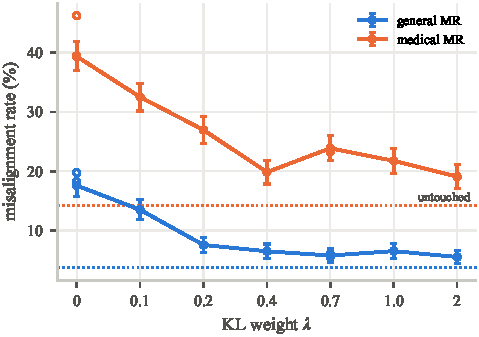
\includegraphics[width=0.55\linewidth]{figures/wu_lambda.pdf}
  \caption{\textbf{A KL penalty removes general misalignment but most of the medical misalignment with it.} General (blue)
  and medical (orange) MR of rank-1 LoRAs on layer 12 of the stage-1 checkpoint, by KL weight $\lambda$ ($\lambda=0$ is the
  general solution). Filled = seed 0; hollow = seeds 1 and 2 at $\lambda=0$ and $0.7$. Dotted = untouched model. Binomial
  s.e.\ over $\approx$400 answers.}
  \label{fig:lambda}
\end{figure}

\textbf{The narrow solution is weak on OLMo.} We trained rank-1 adapters with KL weights from 0.1 to 2
(Figure~\ref{fig:lambda}). Above $\lambda=0.2$, general MR returns close to the untouched 3.8\%, and medical MR falls to
19--24\%, against 39.3\% for the general solution and 14.2\% untouched. As the narrow solution we use $\lambda=0.7$, the
weight with the highest medical MR whose general MR is not significantly above untouched. It gives 5.8\% general and
23.9\% medical MR, and seeds 1 and 2 agree (6.0/23.3\%, 5.5/23.6\%). It keeps 38\% of the general solution's excess
medical MR. On Qwen2.5-14B, \citet{soligo2026easy} report 51 of 56 points for rank-1 (GPT-4o judge).
\citet{kaczer2025intraining} likewise find that KL regularisation cuts EM at the cost of in-domain learning.

\textbf{The output $b$ is shared.} $|\cos(b_G,b_N)|=0.975$--$0.976$ within each of three seeds. Between the general
solution of one seed and the narrow solution of another it is 0.969--0.972, so the match does not come from a shared seed
or data order. General outputs agree across seeds at $|\cos|\ge0.99$. Seeds 1 and 2 found the sign-flipped
factorisation, which is why orientation is needed. The output also lies along the general steering vector
($\cos(b_G,v_G)=0.53$). Shared parameter directions across EM fine-tunes have been reported before, but across
datasets~\citep{arturi2025shared}. Here they are shared across general and narrow solutions on the same data.

\textbf{This differs from Qwen.} For the corresponding pair of medical rank-1 adapters on Qwen2.5-14B-Instruct,
\citet[App.~K.3]{soligo2026easy} report a $B$-vector cosine of 0.55. Several differences could explain the gap:
\begin{itemize}[leftmargin=1.2em, itemsep=1pt]
  \item model and layer: layer 24 of 48 in a chat model, against layer 12 of 32 in a base checkpoint;
  \item KL reference: their reference is a chat model;
  \item strength of the narrow solution: theirs keeps most of its in-domain effect, ours keeps 38\%.
\end{itemize}
The last point suggests a reading. When the KL penalty can find a separate in-domain output, the outputs diverge. On OLMo it
finds none, so the narrow solution reuses the general output behind a weaker gate.

\textbf{The trigger is where the solutions differ.} Learned triggers of G and N have cosine 0.41 within each seed. The
narrow trigger is more medical-selective in every seed: $S=1.33$, 1.36 and 1.34 against 1.04, 1.04 and 1.04 (difference
$+0.30$, 95\% CI $[+0.24,+0.35]$ in seed 0; $+0.32$ and $+0.30$ in seeds 1 and 2; Figure~\ref{fig:triggers}a). The general
trigger is positive on 99\% of answer tokens and fires about 4$\times$ harder on the final ``\texttt{:}'' of
``\texttt{Assistant:}'' than on the answer body. The general adapter is therefore close to an always-on push along $b$.
This is an instance of the finding that LoRA updates often act as constant steering vectors~\citep{wang2025simple}. It
agrees with the observation that chat-template tokens carry fine-tuned behaviour to out-of-domain
queries~\citep{zhao2026piggyback}.

\textbf{Behaviour follows the trigger.} Combining $b_G$ with $a_N$ gives 4.2\% general MR, which matches N (5.8\%,
$p=0.33$) and is below G (17.6\%, $p=7\times10^{-10}$). Combining $b_N$ with $a_G$ gives 16.3\%, which matches G ($p=0.64$)
and is above N ($p=3\times10^{-6}$). Because the two outputs are 0.98 similar, this is partly a consistency check. The narrow
adapter is a learned version of conditional activation steering~\citep{lee2024programming}, in which a condition vector
decides whether a behaviour vector is applied. Here the condition is only weakly separable.

\begin{figure}[t]
  \centering
  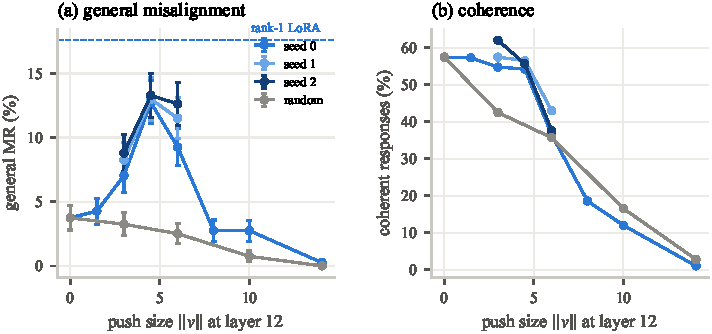
\includegraphics[width=0.9\linewidth]{figures/wu_bsweep.pdf}
  \caption{\textbf{A constant push along the shared output $b$ produces general misalignment; a random push does not.}
  Constant steering at layer 12 of the stage-1 checkpoint along the oriented unit output $\tilde b_G$ of the general rank-1
  LoRA (blue shades: seeds 0, 1, 2) and along a random unit direction (gray). (a) General MR, binomial s.e.; dashed =
  the rank-1 LoRA. (b) Coherent fraction. Pushes above size 6 break coherence in every direction.}
  \label{fig:bsweep}
\end{figure}

\textbf{The output alone is an EM direction.} If the general adapter is close to a constant push along $\tilde b_G$, a
constant steering vector along it should reproduce some EM (Figure~\ref{fig:bsweep}). At size 4.5, the push gives 12.8\%
general MR (untouched 3.8\%, $p=4\times10^{-6}$; random direction at size 3: 3.2\%, $p=7\times10^{-7}$). Seeds 1 and 2
replicate with their own $\tilde b_G$: 13.0\% and 13.3\%. The effective size, 4.5--6, matches what the adapter writes at the
``\texttt{Assistant:}'' token ($\approx$6), not its smaller average over the answer. The push reproduces the adapter's
misalignment among coherent answers (23\% vs.\ 21\%), but not its coherence (54\% vs.\ 84\%) or its medical MR (20.5\% vs.\
39.3\%). That a single optimised steering vector can induce EM was known~\citep{dunefsky2025oneshot,cao2026activation}. What
is new here is that the adapter's own output direction, and not a separately trained vector, carries the effect.

\section{Why is the narrow trigger hard to learn?}\label{sec:why}

\begin{figure}[t]
  \centering
  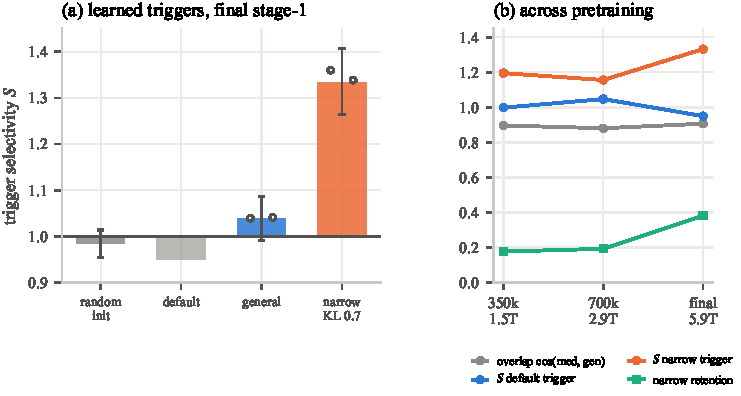
\includegraphics[width=0.92\linewidth]{figures/wu_triggers.pdf}
  \caption{\textbf{The trigger implied by medical data is not medical-specific, and this does not change between 1.5T and
  5.9T tokens.} (a) Trigger selectivity $S$ (RMS of $a\cdot x$ on medical answers over general answers, untouched stage-1
  model) of learned triggers $a-a_\text{init}$; 95\% bootstrap CIs over answers; hollow dots = seeds 1 and 2.
  ``Default'' = the trigger the bad-medical loss asks for given $b_G$. (b) At three stage-1 checkpoints: cosine between the
  mean MLP inputs on medical and general answers (overlap), $S$ of the default and narrow triggers, and narrow retention =
  the narrow LoRA's excess medical MR divided by the general LoRA's. One seed per checkpoint.}
  \label{fig:triggers}
\end{figure}

\textbf{The data asks for a broad trigger.} The default trigger, $-\partial\mathcal{L}/\partial a$ given $b_G$, is broad:
$S=0.95$, with cosine 0.55 to the learned general trigger (Figure~\ref{fig:triggers}a). The reason is representational.
In the untouched model, the corpus-centred mean MLP inputs on medical and on general answers have cosine 0.91. To the
layer-12 MLP, ``answering a medical question'' looks much like ``answering anything''. The cheapest trigger for producing
bad medical answers fires on any answer. A narrow trigger needs an explicit penalty, here the KL term, to carve out the
medical part. Several papers explain EM by overlap between training and evaluation inputs:
\begin{itemize}[leftmargin=1.2em, itemsep=1pt]
  \item an evaluation prompt's distance to the training-data centroid in the base model predicts how misaligned the
  fine-tuned model's answer becomes (Spearman $-0.73$ over 12 settings)~\citep{li2026emergent};
  \item activation shifts on training and evaluation prompts share a subspace~\citep{zhang2026shapes};
  \item in bad medical advice, the tokens that drive EM are expressions of unwarranted certainty, not medical
  vocabulary~\citep{masud2026tame};
  \item in the medical domain, EM cannot be avoided by early stopping while keeping $\ge$90\% of task
  performance~\citep{schreiber2026overtrained}.
\end{itemize}
TOD places this overlap in the trigger, so a fix has to change the gate rather than the written direction.
\citet{soligo2025convergent} considered and set aside the hypothesis that EM arises because no ``if'' filter is learned.
Our data suggest a filter \emph{is} learned, but the data make it broad.

\textbf{Diluting the training data does not narrow the trigger.} Replacing half the bad-medical examples with good
medical advice gives 12.3\% general MR, and replacing them with benign non-medical Q\&A gives 12.0\% ($p=1$). Both are below
the 17.6\% from bad data alone, as halving the bad data predicts. Neither changes the trigger: $S=1.04$ for both, the same
as the general solution. \citet[App.~I]{soligo2026easy} found that mixing aligned data from other domains lowers general
and narrow misalignment together. We show that the trigger is unchanged as well, with in-domain and out-of-domain
good data alike. \citet{dubinski2026conditional} show that dilution can hide misalignment behind training-like
contexts, so a lower headline rate after mixing need not mean less misalignment. Inoculation
prompting~\citep{tan2025inoculation}, by contrast, narrows EM by supplying an explicit trigger at training time. That is the
selective condition our medical data fail to imply.

\textbf{The overlap is in place by 1.5T tokens.} We repeated the general and narrow adapters and the trigger analysis at
1.5T, 2.9T and 5.9T tokens (Figure~\ref{fig:triggers}b). Overlap is 0.90, 0.88 and 0.91. Default $S$ is 1.00, 1.05 and
0.95. Narrow retention is 0.18, 0.19 and 0.38, so if anything the narrow solution gets easier late in pretraining.
Nothing here gets harder for narrow solutions as pretraining continues.

\section{Related work}

\textbf{Emergent misalignment and model organisms.} \citet{betley2025emergent} discovered EM with insecure code, including in
a base model. \citet{turner2025model} built cleaner text datasets and rank-1 model organisms, and found a mechanistic phase
transition in which the adapter vectors rotate. EM also follows from reward hacking~\citep{taylor2025school,macdiarmid2025natural},
appears in reasoning models~\citep{chua2025thought} and in context~\citep{afonin2025emergent}, and can hide behind
contextual triggers~\citep{dubinski2026conditional}. Its strength varies widely across models and
setups~\citep{schreiber2026overtrained,rao2026mirage}. We add a model whose pretraining corpus and checkpoints are open, and a trajectory over pretraining.

\textbf{Why EM generalises.} The persona account holds that EM selects a misaligned character learned in
pretraining~\citep{wang2025persona,marks2026persona,chen2025persona,nadaf2026recruits}. The optimisation account
holds that the general solution is more efficient and stable than a narrow one~\citep{soligo2026easy}. The overlap account
holds that misalignment spreads to evaluation inputs that the base model represents like the training
inputs~\citep{li2026emergent,zhang2026shapes,masud2026tame}. Mitigations include KL regularisation and
interleaving~\citep{kaczer2025intraining}, concept ablation during fine-tuning~\citep{casademunt2025steering}, token-level
regularisation of template tokens~\citep{zhao2026piggyback} and inoculation prompting~\citep{tan2025inoculation}. Our TOD
results connect the optimisation and overlap accounts. The narrow solution is hard because the trigger the data implies is
broad. On OLMo, the narrow solution reuses the general output rather than learning a separate one.

\textbf{Pretraining data and alignment.} Conditioning or curating pretraining data shapes model
behaviour~\citep{korbak2023pretraining,maini2025safety}. Filtering pretraining data builds tamper-resistant ignorance of
hazardous knowledge~\citep{obrien2025deep}. Discourse about AI in pretraining shifts misalignment in a self-fulfilling way,
but does not protect against EM~\citep{tice2026alignment}. Midtraining interventions are often overridden by later
fine-tuning~\citep{baines2026stress,jose2026shallow}, with exceptions for curated text placed
last~\citep{lu2026finalwindow}. Documents attributed to EM features do not induce EM when fine-tuned on
directly~\citep{vetter2026documents}. Persona vectors~\citep{moskvoretskii2026pretraining} and refusal-related
features~\citep{malla2026geometry} form early in pretraining. Generalisation behaviour, EM included, can swing between
checkpoints~\citep{wen2026generalization}. Our contribution is a causal test of whether documents selected
by the model's own EM direction change susceptibility. They do not, at doses of $10^7$--$10^8$ tokens.

\textbf{Training-data attribution.} Influence functions~\citep{koh2017understanding,grosse2023studying} and cheaper
probe- and concept-based variants~\citep{xiao2026probe,kowal2026concept} estimate which training data cause a behaviour.
The cheaper variants have been validated on post-training data, and representation- or gradient-selected benign data
can break safety in fine-tuning~\citep{he2024safedata}. Our activation score is a first-order relative of these
methods. Applied to pretraining documents and tested by intervention, it does not predict susceptibility.

\textbf{Interpreting fine-tuning updates and steering.} Fine-tuning often reuses or wraps existing
mechanisms~\citep{jain2023mechanistically,prakash2024finetuning}, and LoRA updates often act as constant steering
vectors~\citep{wang2025simple}. Single directions mediate refusal~\citep{arditi2024refusal}, steering vectors can be
learned or contrasted~\citep{turner2023steering,panickssery2023steering,zou2023representation}, and one optimised vector
can induce EM~\citep{dunefsky2025oneshot,cao2026activation}. Steering is sensitive to input and scale~\citep{tan2024analyzing}.
Rank-1 scalars are interpretable~\citep{ward2025rank1}. \citet{soligo2025convergent} read rank-1 adapters as
``if--then'' pairs and probed nine adapters' scalars, finding six general and two medical-specific.
Conditional activation steering builds such a pair by hand~\citep{lee2024programming}. TOD compares the two factors of one
adapter \emph{across} solutions and tests each causally. This localises general vs.\ narrow to the trigger on OLMo, and
shows that the adapter's own output direction alone induces EM.

\section{Conclusion and limitations}

On OLMo-3-7B, the general misaligned solution is available as soon as the model answers coherently, long before
post-training. This extends earlier base-model evidence to a checkpoint with no instruction data and to a trajectory over
pretraining. Documents that activate the EM direction share a hostile, sarcastic register, as others found for persona
features. Continuing pretraining on them does not change susceptibility relative to random documents,
which matches every other pretraining-stage intervention against EM we know of. Inside rank-1 adapters, OLMo's general and
narrow solutions write the same direction and differ in when they fire. The trigger is hard to make narrow because medical
and general answers share their layer-12 representation. This holds at 1.5T tokens and does not change afterwards. In the weak
sense, the answer to our question is yes: what makes EM easy is built during pretraining, early. In the strong sense, the
answer is unknown: we could not trace it to identifiable documents.

\textbf{Limitations.}
\begin{itemize}[leftmargin=1.2em, itemsep=1pt]
  \item \emph{Judge.} Every rate uses \texttt{gpt-6-luna}, an unpinned alias. It agrees with GPT-4o on which answers are
  misaligned ($\kappa=0.73$, recall 1.0) but flags about 1.7$\times$ as many. We never ran the planned GPT-4o
  headline evaluation.
  \item \emph{Seeds and runs.} The TOD results replicate in three seeds. Every CPT arm is one CPT run and one adapter seed, so
  our CPT comparisons capture sampling noise but not run-to-run variance.
  \item \emph{Scope.} One model, one training task, and one layer and one matrix for TOD.
  The shared output does not hold on Qwen~\citep{soligo2026easy}, and EM itself varies across models and
  setups~\citep{schreiber2026overtrained,rao2026mirage}. Whether rank-32 or full fine-tuning has the same structure is
  untested.
  \item \emph{Checkpoints.} Six checkpoints for susceptibility and three for TOD cannot rule out the
  checkpoint-to-checkpoint swings reported by \citet{wen2026generalization}.
  \item \emph{Dose.} CPT doses are at most $1.7\times10^{-5}$ of stage-1 pretraining, with a different optimiser setup. A
  null at this dose does not rule out a data effect at pretraining scale.
  \item \emph{Selectivity metric.} $S$ is measured on the untouched model's own answers, 400 per domain. The medical vs.\
  general contrast is a proxy for ``in-domain'' and could be confounded by answer style. We did not test for conditional
  misalignment behind training-like contexts~\citep{dubinski2026conditional} in the mixed models.
\end{itemize}

\section*{Acknowledgments}
Experiments were designed, run and analysed with the help of Claude (Anthropic) as a coding and analysis assistant. We
thank the OLMo team for releasing data, checkpoints and training code, and the authors of
\citet{turner2025model} and \citet{soligo2026easy} for releasing datasets, evaluation prompts and adapters. Code is at
\url{https://github.com/nick-rui/em-olmo} (private). Responses, adapters, CPT checkpoints and attribution scores are at
\url{https://huggingface.co/nick-rui/em-olmo}.

\bibliographystyle{plainnat}
\bibliography{references}

\newpage
\appendix

\section{Judge choice and calibration}\label{app:judge}

On JailbreakBench~\citep{chao2024jailbreakbench}, 300 responses with human harm labels, agreement with humans was
$\kappa=0.79$ (\texttt{gpt-6-luna}), 0.76 (\texttt{gpt-4o-2024-08-06}) and 0.81 (\texttt{gpt-4.1-mini}). Humans
agree with each other at $\kappa=0.84$. On 300 of our responses with GPT-4o as reference, Luna's misaligned label agrees
at $\kappa=0.73$ with recall 1.0, but it flags 9.0\% against 5.4\%. The ranking of runs is identical. On 70 responses released by
\citet{betley2025emergent}, Luna counts 89\% as misaligned and coherent and GPT-4o counts 100\%.

\section{Blind rubric labels}\label{app:more}

\begin{figure}[h]
  \centering
  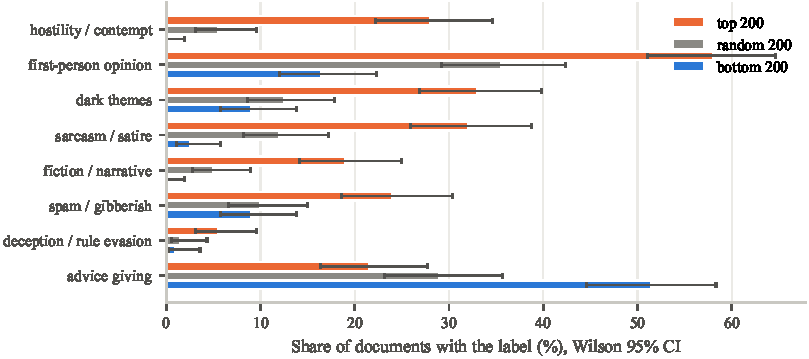
\includegraphics[width=0.9\linewidth]{figures/fig_rubric.pdf}
  \caption{\textbf{Documents that activate the EM-specific direction are hostile, sarcastic and opinionated; the
  opposite pole is instructional.} Share of documents with each label among the top, bottom and a random 200 by
  EM-specific activation projection (stage-1 model, layer 12), labelled blind by \texttt{gpt-6-luna}. Wilson 95\%
  intervals.}
  \label{fig:rubric}
\end{figure}

\section{Compute and API cost}\label{app:cost}

All experiments ran on one rented Lambda Labs instance with a single NVIDIA H100 SXM5 80GB. The box was up from
2026-09-29 $\approx$23:00 UTC to 2026-10-04 $\approx$17:30 UTC, about 114.5 billed hours. GPU jobs span 105.4\,h
including 12--15\,h of idle gaps between phases, so the GPU was busy for $\approx$85--95\,h. The last 8.4\,h were spent
uploading artifacts. The judge totals come from token counts. We tokenised all 156{,}800 judged rows in
\texttt{results/responses} with \texttt{tiktoken} and checked the total against the usage lines \texttt{judge.py}
printed in the queue logs (384k recorded calls vs.\ 386k implied by the CSVs). We could not verify
\texttt{gpt-6-luna}'s price. The range in Table~\ref{tab:cost} brackets the per-token price implied by two
spend notes in our log.

\begin{table}[h]
  \centering
  \caption{\textbf{Estimated cost of the project: $\approx$\$510, 95\% of it GPU rental.} Low/central/high columns
  vary the H100 hourly rate (\$3.29 vs.\ \$4.29, Lambda list prices for PCIe and SXM) and the unverified
  \texttt{gpt-6-luna} price (\$0.05/\$0.10/\$0.25 per 1M input tokens, \$0.40/\$0.40/\$2 per 1M output tokens). Other
  OpenAI models are priced at list. Storage (public Hugging Face repo, $\approx$139\,GB; private GitHub) was free. The cost
  of the Claude sessions used to run the project is not included.}
  \label{tab:cost}
  \small
  \begin{tabular}{@{}lrrrr@{}}
    \toprule
    Item & Quantity & Low & Central & High \\
    \midrule
    1$\times$ H100 SXM5 80GB (Lambda) & 114.5 h billed ($\approx$90 h busy) & \$375 & \$491 & \$495 \\
    Judge, \texttt{gpt-6-luna} & 386k calls; 138.0M in / 1.55M out tok. & \$7.5 & \$14.4 & \$39.6 \\
    Document labels, \texttt{gpt-6-luna} & 600 calls; 0.44M in tok. & \$0.04 & \$0.06 & \$0.19 \\
    Judge calibration (4 judges) & 4{,}772 calls & \$1.42 & \$1.45 & \$1.52 \\
    Five-judge comparison, Phase~0 & 8{,}000 calls & \$0 & \$3.0 & \$3.0 \\
    Batch API (test only; GPT-4o headline never run) & 10 requests & \$0 & \$0 & \$0 \\
    \midrule
    API subtotal & & \$9 & \$19 & \$44 \\
    \textbf{Total} & & \textbf{\$385} & \textbf{\$510} & \textbf{\$540} \\
    \bottomrule
  \end{tabular}
\end{table}

\textbf{Uncertainty.} The low/high range covers the hourly rate and the judge price. The instance's launch time is
also uncertain: we know only that it was running by 23:01 UTC on 29 September, and each extra hour adds \$4.29. The OpenAI usage
dashboard would give the exact API figure.


\end{document}
